\documentclass{beamer}
\mode<presentation> {

\usetheme{Singapore}
\setbeamertemplate{footline}[page number]
}

\usepackage{graphicx} % Allows including images
\usepackage{booktabs} % Allows the use of \toprule, \midrule and \bottomrule in tables


\title[Short title]{Feeder: An all purpose academic App} 
\author{Alpha (Group 20)} % Your name
\institute[IIT Bombay]
{
IIT Bombay \\ % Your institution for the title page
\medskip
}
\date{\today}

\begin{document}

\begin{frame}
\titlepage % Print the title page as the first slide
\end{frame}

\begin{frame}
\frametitle{Overview} 
\tableofcontents
\end{frame}

%----------------------------------------------------------------------------------------
%	PRESENTATION SLIDES
%----------------------------------------------------------------------------------------

%------------------------------------------------
\section{Introduction}

\begin{frame}
\frametitle{Introduction}
Feeder is the app every college should adopt for the students. In short the app serves 2 basic things:
\begin{itemize}
\item For Students: It provides a personalized dynamic academic timetable. With so many deadlines for different courses an app to serve as a reminder for all academic puroposes is a very good option.
\item For Professors: To provide good quality education it is important to have regular feedbacks. Also in todays world with almost every student uses a smartpohone and thus its easy to give feedback per module covered, per exam, per test. Feeder provides a platform to make this happen.
\end{itemize}
Overall it is a perfect tool to help both professors and students.
\end{frame}

%------------------------------------------------
\section{Web App}

\begin{frame}
\frametitle{Web App}
\begin{itemize}
\item The web application is administered by professor.
\item It provides platform to professors to add feedback forms and deadlines which students can view on the mobiles.
\item Professor can check feedback in really helpful format with help of graphs.
\end{itemize}
\begin{figure}[ht!]
    \centering
      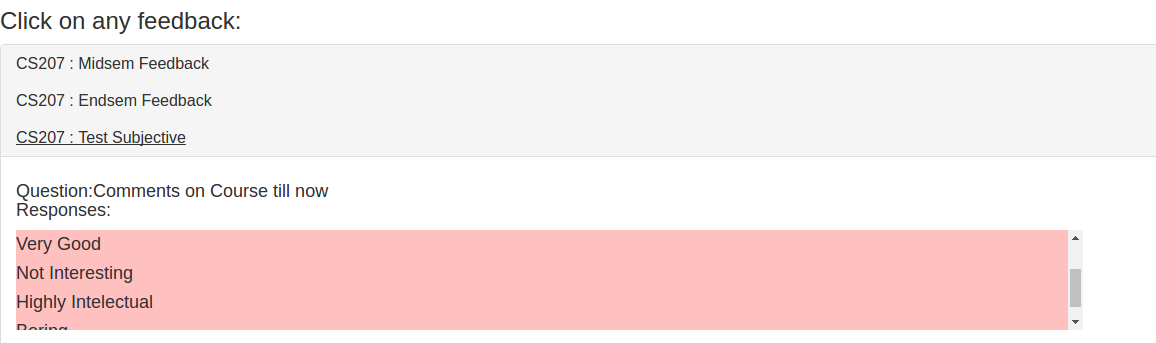
\includegraphics[width=.4\linewidth]{images/subjectiveAnswers.png}
      \caption{View Feedback\label{overflow}}
  \end{figure}
\end{frame}

%------------------------------------------------
\section{Android App}

\begin{frame}
\frametitle{Android App}
\begin{itemize}
\item The Android App is meant for the students.
\item It provides platform to student to view feedback forms and assignment deadlines.
\item It has a very friendly UI with use of different colors for different courses.
\end{itemize}
\begin{figure}[ht!]
    \centering
      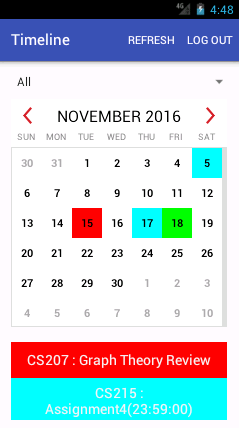
\includegraphics[width=2.5cm,height=4cm]{images/calendarMix.png}
      \caption{Calendar View\label{overflow}}
  \end{figure}
\end{frame}
%------------------------------------------------

\begin{frame}
\Huge{\centerline{The End}}
\end{frame}

%----------------------------------------------------------------------------------------
\end{document} 